% NAME: S322517454张云涛作业
\documentclass{article}
\usepackage{ctex}
\usepackage{listings}
\usepackage{xcolor}
\usepackage{pdfpages}
\usepackage{graphicx}
\usepackage{geometry}
\usepackage{float}
\usepackage{amsmath}
\usepackage{hyperref}
\usepackage{fontspec}
\usepackage{anyfontsize}
\usepackage[version=4]{mhchem}     % 化学公式用
\usepackage{graphicx}
\usepackage{subfigure}
\usepackage{pdfpages}
\usepackage{titlesec} %自定义多级标题格式的宏包
\usepackage{fancyhdr}
\titleformat{\section}[block]{\LARGE\bfseries}{题目\arabic{section}}{0em}{: }[]

\geometry{a4paper, left=2cm, right=2cm, top=1cm, bottom=2cm}

\lstset{
	%backgroundcolor=\color{red!50!green!50!blue!50},%代码块背景色为浅灰色
%	rulesepcolor= \color{gray}, %代码块边框颜色
	breaklines=true,  %代码过长则换行
	numbers=left, %行号在左侧显示
	numberstyle= \small,%行号字体
	keywordstyle= \color{blue},%关键字颜色
	commentstyle=\color{gray}, %注释颜色
%	frame=shadowbox%用方框框住代码块
	frame=single,
    showstringspaces = false,
    basicstyle=\ttfamily,
	escapeinside=``    % 代码包含中文
}

\begin{document}

\includepdf[pages={1}]{相关资源/封面.pdf} 

\section{插值} 
\subsection{摘要}
美国人口普查美10年一次,下表列出了1960年到2020年到人口(按千人计)。
\begin{table}[!ht]
    \centering
    \begin{tabular}{|c|c|c|c|c|c|c|c|}
    \hline
        年 & 1960年 & 1970年 & 1980年 & 1990年 & 2000年 & 2010年 & 2020年 \\ \hline
        人口(千) & 180 671 & 205 052 & 227 225 & 249 623 & 282 162 & 309 327 & 329 484 \\ \hline
    \end{tabular}
\end{table}
\begin{enumerate}
    \item 用适当Lagrange插值法分别求在1950年、2005年和2030年人口的近似值。
    \item 1950年的人口大约是151326(千人),
        你认为你得到的2005年(据查295,516千人)
        和2030年(预测)的人口数字精确度如何?
    \item 用适当Newton插值法重做1.1和1.2 
    \item 使用适当自由三次样条插值法重做1.1和1.2
\end{enumerate}

\subsection{数学原理}
\subsubsection{Lagrange插值}
\begin{align}
    L_n(x) & = \sum_{k=0}^{n}y_k\frac{w_{n+1}(x)}{(x-x_k)w'_{n+1}(x_k)} \\
    R_n(x) & = \frac{1}{n+1}f^{(n+1)}(\eta)w_{n+1}(x) \\
    w_{n+1}(x) & = \mathop{\Pi}\limits_{i=0}^n (x-x_i) 
\end{align}

\subsubsection{Newton插值}
\begin{align}
    P_n(x) = & f(x_0) + f[x_0, x_1](x-x_0) + f[x0_0, x_1, x_2](x-x_0)(x-x_1)(x-x_2) + \cdots \nonumber \\ 
    & + f[x_0, x_1, ,\cdots, x_n](x-x_0)\cdots(x-x_n) \\
    R_n(x) = & f[x, x_0, \cdots, x_n]w_{n+1}(x) \\
    f[x_0,x_1,\cdots,x_k] = & 
        \frac{f[x_0,x_1,\cdots,x_{k-2},x_k]-f[x_0,x_1,\cdots,x_{k-1}]}{x_k-x_{k-1}} 
        \hspace*{1cm}, \text{均差} 
\end{align}

\subsubsection{三次样条}
若函数$S(x)\in C^2[a,b]$,且每个小区间上$[x_j,x_{j+1}]$上是三次多项式,
其中$a=x_0<x_1<\cdots<x_n=b$为给定节点,则称$S(x)$为
节点$x_0,x_1,\cdots,x_n$上的三次样条函数。

\subsubsection{相对误差}
\begin{align}
    e_r^* = \frac{e^*}{x} = \frac{x-x^*}{x}
\end{align}
\subsection{程序设计}
\lstinputlisting[language=Python,caption={from:源代码/题目1插值},captionpos=b, firstline=1, lastline=58]{源代码/题目1插值.py}

\subsection{结果分析}
\begin{figure}[H]
    \centering
    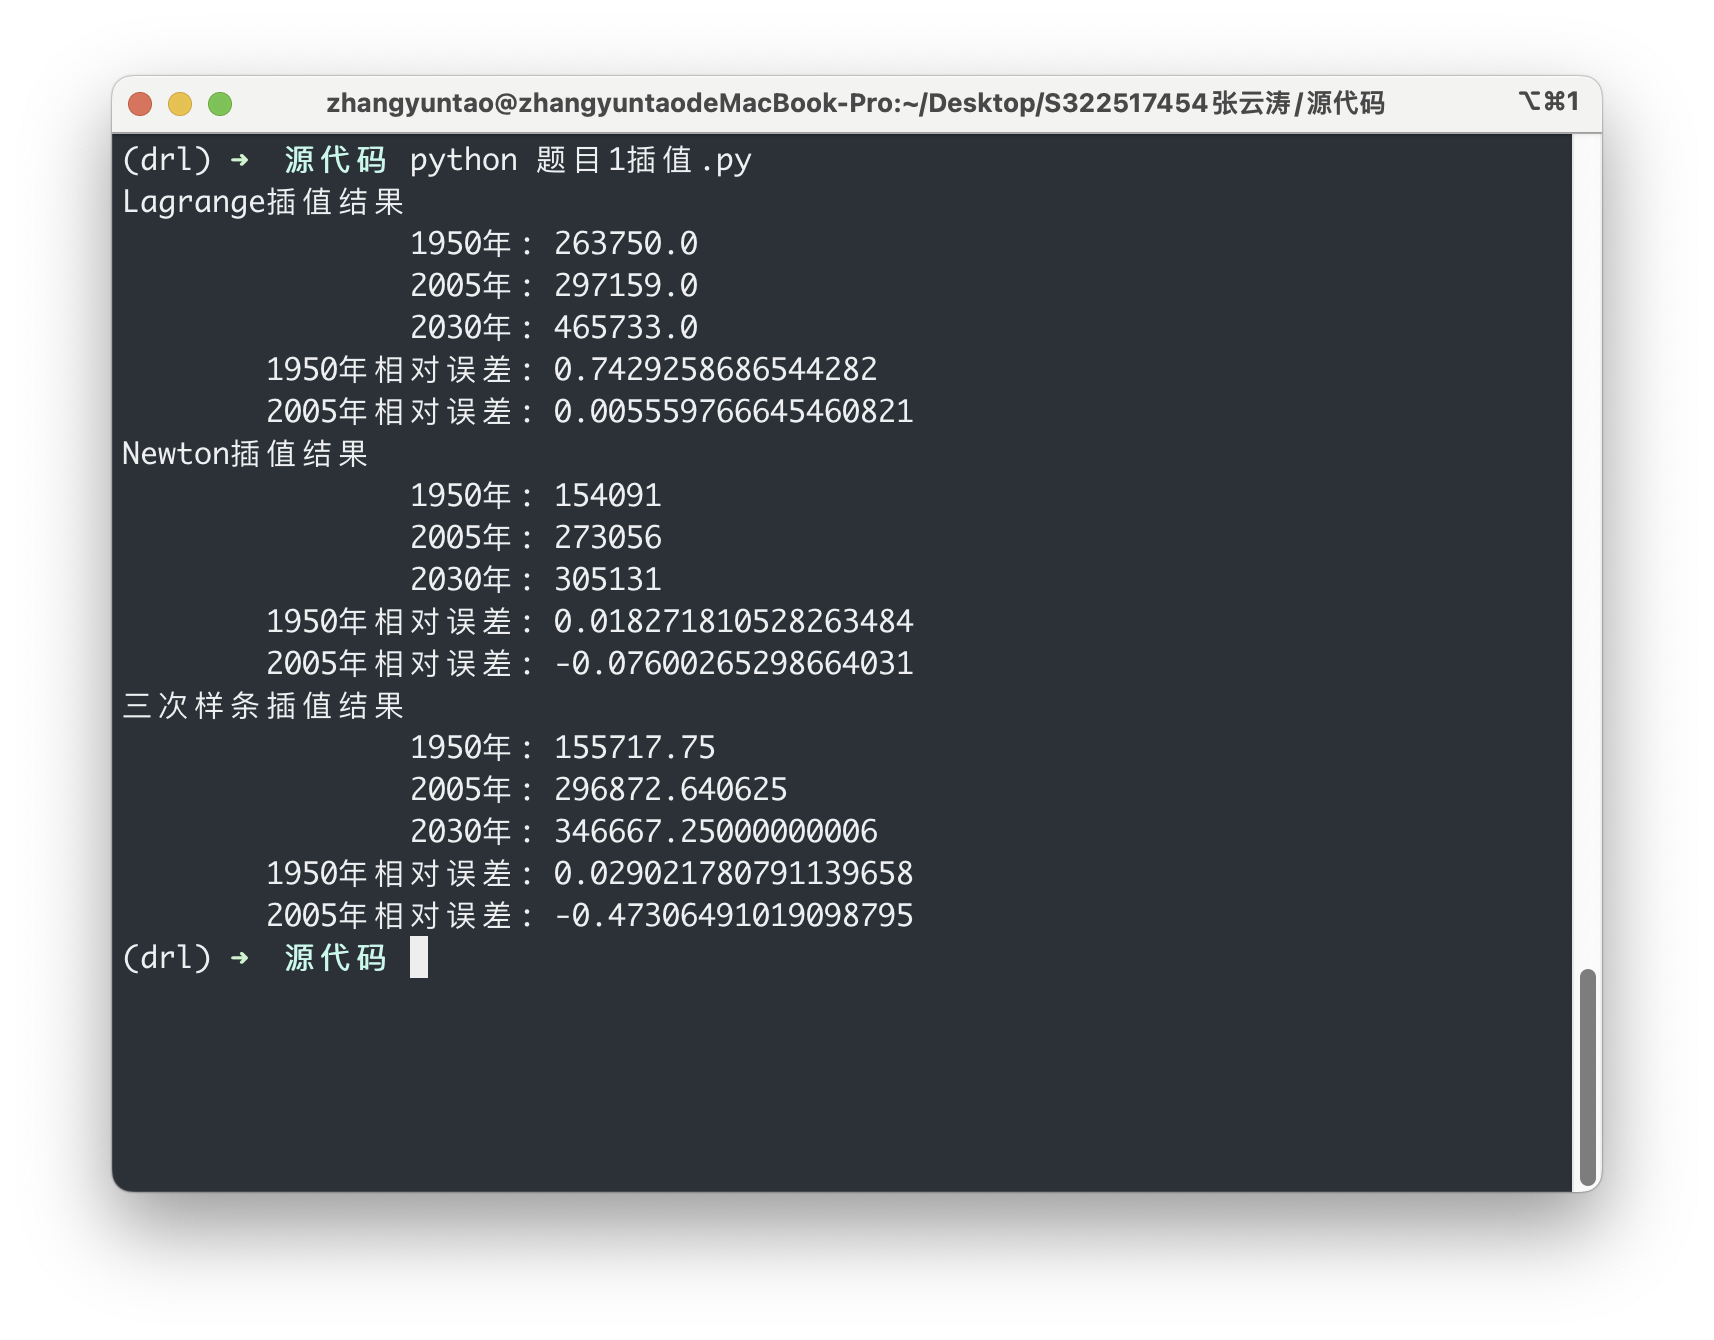
\includegraphics[width=\textwidth]{相关资源/图片/题目1插值运行结果.png} 
\end{figure}

\begin{table}[H]
    \centering
    \begin{tabular}{|c|c|c|c|c|c|c|}
    \hline
        年份 & Lagrange插值 & 误差 & Newton插值 & 误差 & 三次样条插值 & 误差 \\ \hline
        1950年 & 263750 & 0.742925869 & 154091 & 0.018271811 & 155717.75 & 0.029021781 \\ \hline
        2005年 & 297159 & 0.005559767 & 273056 & -0.076002653 & 296872.6406 & -0.47306491 \\ \hline
        2030年 & 465733 & ~ & 305131 & ~ & 346667.25 & \\ \hline
    \end{tabular}
\end{table}

Lagrange插值1950年插值结果误差较大,2005年插值结果误差小,可见出现了龙格现象,导致边界处插值结果不准确。
需要考虑采用低次Lagrange插值控制边界处插值误差。

\subsection{体会与收获}
插值方法原理清晰,但是编程实现还是有一定难度,因此Lagrange插值和三次样条插值
都是直接调用python的scipy包进行实现。自己的编程能力还需要不断提升。
理解了常用插值方法的基本原理,并且熟悉了插值库的使用方法,还是获益匪浅的。

%%%%%%%%%%%%%%%%%%%%%%%%%%%%%%%%%%%%%%%%%%%%%%%%%%%%%%%%%%%%%%%%%%%%%%%%%%%%%%
\newpage
\section{拟合}
\subsection{摘要}
生物学家在研究天蛾幼虫的生长时采用了下面的数据确定$w$
(活幼虫的重量,以克计算)和$R$(幼虫消耗的氧气,以毫升/小时计算)之
间的关系$R=bw^3$。
\begin{table}[!ht]
    \centering
    \begin{tabular}{|c|c|c|c|c|c|c|c|c|c|}
    \hline
        w & R & w & R & w & R & w & R & w & R \\ \hline
        0.017 & 0.154 & 0.174 & 0.363 & 1.29 & 0.87 & 3.04 & 3.59 & 4.83 & 4.66 \\ \hline
        0.02 & 0.181 & 0.210  & 0.428 & 1.32 & 1.15 & 3.34 & 2.83 & 5.30  & 3.88 \\ \hline
        0.025 & 0.234 & 0.211 & 0.366 & 1.35 & 2.48 & 4.09 & 3.58 & 5.45 & 3.52 \\ \hline
        0.085 & 0.26 & 0.233 & 0.537 & 1.69 & 1.44 & 4.28 & 3.28 & 5.48 & 4.15 \\ \hline
        0.087 & 0.296 & 0.783 & 1.47 & 1.74 & 2.23 & 4.29 & 3.40  & 5.53 & 6.94 \\ \hline
        0.119 & 0.299 & 0.999 & 0.771 & 2.75 & 1.84 & 4.58 & 2.96 & 5.96 & 2.40  \\ \hline
        0.171 & 0.334 & 1.11 & 0.531 & 3.02 & 2.01 & 4.68 & 5.10 & & \\ \hline
    \end{tabular}
\end{table}
\begin{enumerate}
    \item 利用对数最小二乘方程\texorpdfstring{$\ln R=\ln b+a\ln w$}{}拟合,
        确定参数\texorpdfstring{$a,b$}{}。
    \item 计算2.1中的平方误差
    \item 修改2.1中的对数最小二乘方程\texorpdfstring{$\ln R=\ln b+a\ln w+c(\ln w)^2$}{},
        确定参数\texorpdfstring{$a,b,c$}{} 
\end{enumerate}

\subsection{数学原理}
\subsubsection{最小二乘法拟合}
根据需要拟合的多项式$S(x)=a_0+a_1x+\cdots+a_nx^n$,
选择正交多项式基底
$\varphi=span\{1,x,x^2,\cdots,x^n\}$。\\
建立法方程
\begin{equation}
    Ga = d 
\end{equation}
\begin{align}
    G = &
    \begin{pmatrix} 
        (\varphi_0,\varphi_0) & (\varphi_0,\varphi_1) & \cdots & (\varphi_0,\varphi_n) \\
        (\varphi_1,\varphi_0) & (\varphi_1,\varphi_1) & \cdots & (\varphi_1,\varphi_n) \\
        \vdots & \vdots & \ddots & \vdots \\
        (\varphi_n,\varphi_0) & (\varphi_n,\varphi_1) & \cdots & (\varphi_n,\varphi_n) \\
    \end{pmatrix} \\
    a = & (a_0, a_1, \cdots, a_n)^T \\
    d = & (d_0, d_1, \cdots, d_n)^T = 
    \begin{pmatrix}
        (f,\varphi_0) \\
        (f,\varphi_1) \\
        \vdots \\
        (f,\varphi_n)
    \end{pmatrix} 
\end{align}
其中
\begin{align}
    (\varphi_j, \varphi_k) = & \sum_{i=0}^m\varphi_j(x_i)\varphi_k(x_i) \\
    (f, \varphi_k) = & \sum_{i=0}^mf(x_i)\varphi_k(x_i) 
\end{align}
对于某些计算较为复杂的情形,比如本题,考虑对等式两边取对数,
如$\ln R = \ln b + a\ln w$。
\subsubsection{平方误差}
\begin{align}
    ||\delta||_2^2 = & \min_{S(x)\in\varphi} \sum_{i=0}^{m}[S(x_i)-y_i]^2 \\
    S(x) = & a_0\varphi_0(x) + a_1\varphi_1(x) + \cdots + a_n\varphi_n(x) 
\end{align}
\subsection{程序设计}
\lstinputlisting[language=Python,caption={from:源代码/题目2拟合},captionpos=b, firstline=1, lastline=66]{源代码/题目2拟合.py}

\subsection{结果分析}
\begin{figure}[H]
    \centering
    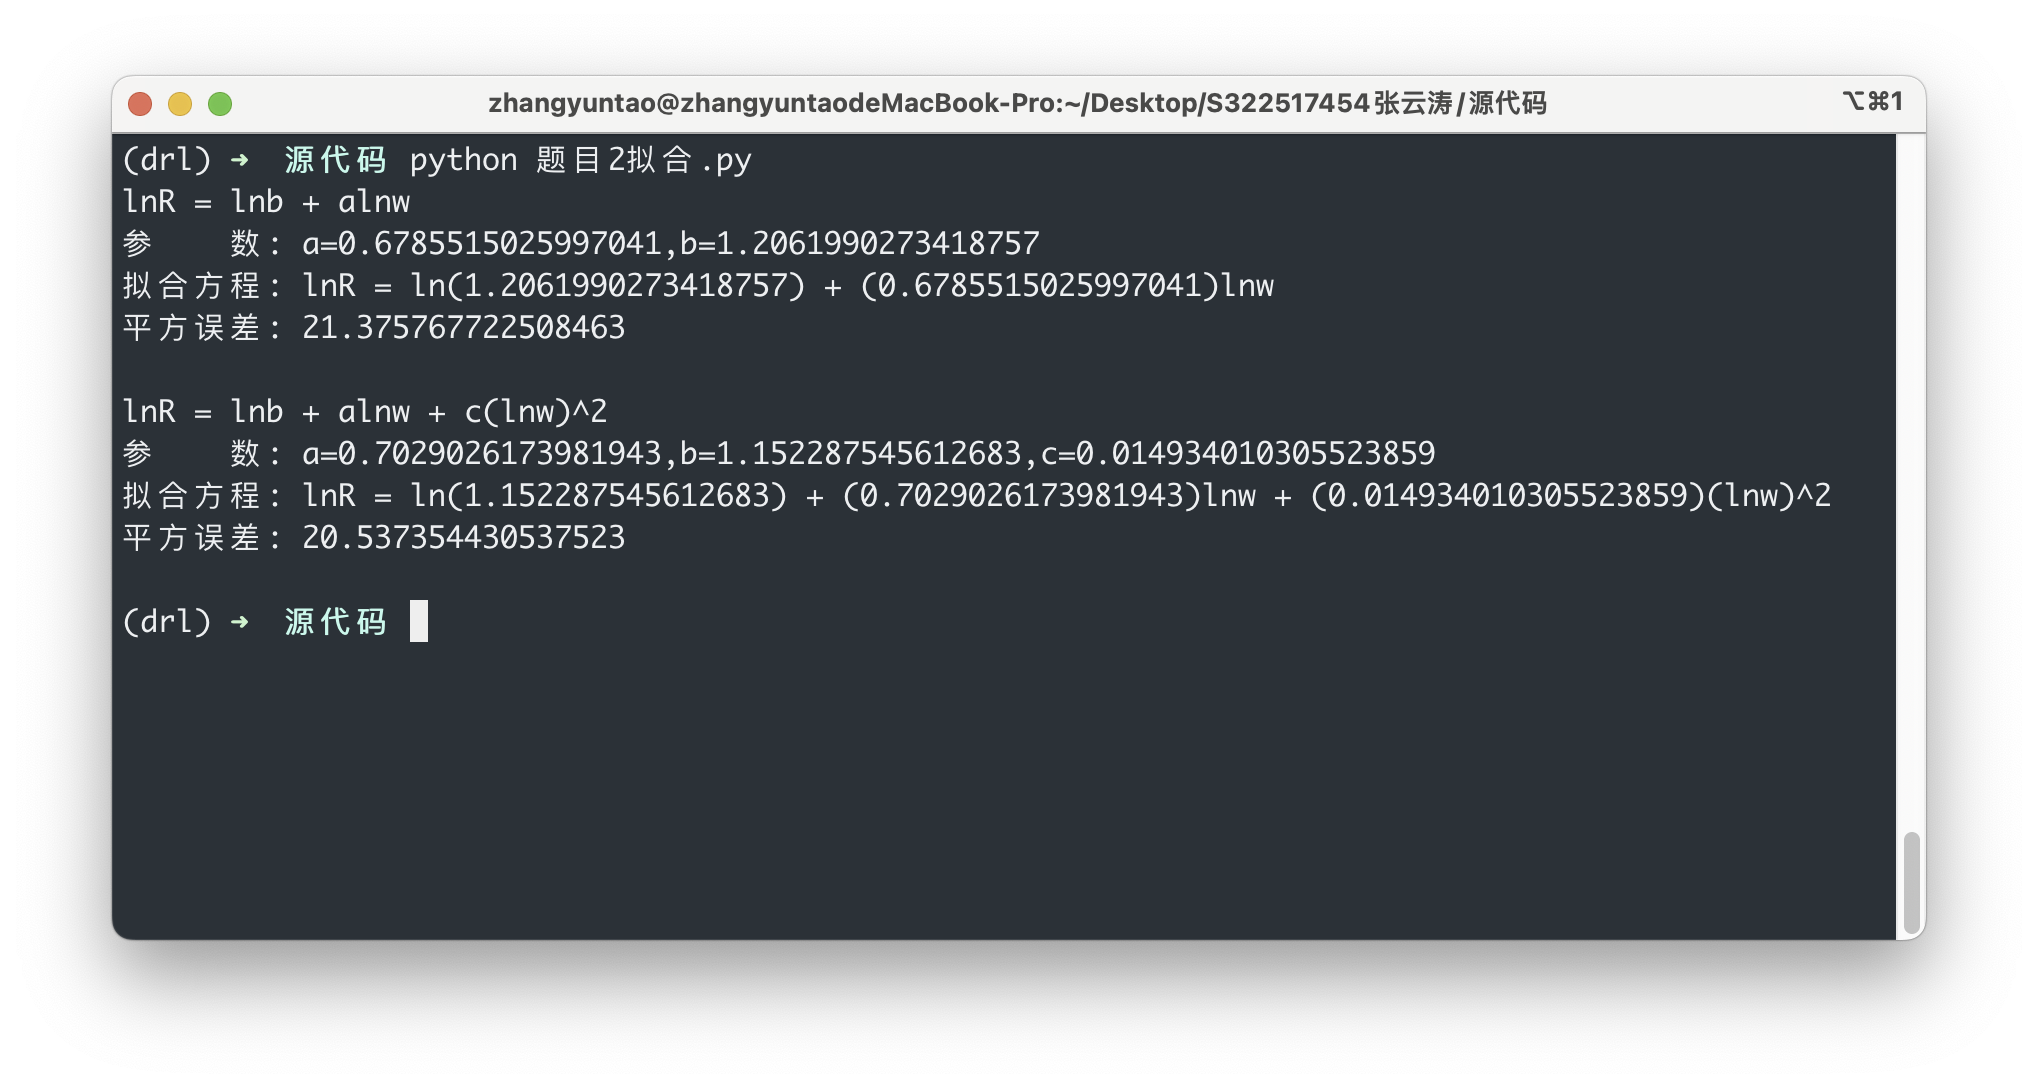
\includegraphics[width=\textwidth]{相关资源/图片/题目2拟合运行结果.png} 
\end{figure}
关于对数最小二乘
方程$\ln R = \ln b + a\ln w$,解得 \\
拟合方程为$\ln R=\ln(1.2814949827597537)+(0.5975089923633367)\ln w$,\\
参数$a=0.5975089923633367,b=1.2814949827597537$。\\
平方误差为24.29908840924062。 \\ 

关于对数最小二乘方程$\ln R=\ln b+a\ln w+c(\ln w)^2$,解得 \\
拟合方程为$\ln R=\ln(1.0459951729587154)+(0.7056490814343211)\ln w+(0.06631997011335665)(\ln w)^2$,\\
参数为$a=0.7056490814343211,b=1.0459951729587154,c=0.06631997011335665$,\\
平方误差为: 20.294731547887828。

\subsection{体会与收获}
最小二乘拟合是日常工作生活中使用频率很高的算法,之前的工作中也多次使用,
通过这一次的学习和实验,得以进一步巩固,我可以在今后更加熟练的加以运用。

%%%%%%%%%%%%%%%%%%%%%%%%%%%%%%%%%%%%%%%%%%%%%%%%%%%%%%%%%%%%%%%%%%%%%%%%%%
\newpage
\section{非线形方程求根与数值积分综合}
\subsection{摘要}
求非线形方程
$\int_0^x\frac{1}{\sqrt{2\pi}}e^{-\frac{t^2}{2}}dt=0.45$时,
令
\begin{equation}
    f(x) = \int_0^x\frac{1}{\sqrt{2\pi}}e^{-\frac{t^2}{2}}dt - 0.45    
\end{equation}
若利用Newton迭代格式,需要用到计算各迭代节点的积分值
$\int_0^{x_k}\frac{1}{\sqrt{2\pi}}e^{-\frac{t^2}{2}}dt$。

\begin{enumerate}
    \item 用Romberg求积计算迭代需要的各项积分值
    \item 用Gauss-Legendre三点公式计算迭代所需要的各项积分值
    \item 取初值\texorpdfstring{$x_0=0.5$}{},
        选取3.1或3.2的各节点积分值,用Newton迭代法
        求得改非线形方程的根
\end{enumerate}

\subsection{数学原理}

\begin{align}
    \text{Newton迭代} & \nonumber \\
    x_{k+1} & = x_k + \frac{f(x_k)}{f'(x_k)} \\
    \text{Romberg求积} & \nonumber \\
    T_{2n} & = \frac{1}{2}T_n + \frac{h}{2}\sum_{k=0}^{n-1}f(x_{k+\frac{1}{2}}) \\
    T_m^{(k)} & = \frac{4^m}{4^m-1}T_{m-1}{(k+1)}-\frac{1}{4^m-1}T_{m-1}^{(k)} \\
    \text{Gauss-Legendre求积} & \nonumber \\
    \int_{-1}^1f(x)dx & \approx \frac{5}{9}f(-\frac{\sqrt{15}}{5})+\frac{8}{9}f(0)+\frac{5}{9}f(\frac{\sqrt{15}}{5}) \\
    \text{区间变换,映射到}[-1,1] & \nonumber \\
    x & = \frac{1}{2}[(b-a)t+a+b]  \\
    % Y & = Y_{min} + \frac{Y_{max} - Y_{min}}{X_{max}-X_{min}}(X-X_{min})
    \text{Gauss-Legendre求积} & \nonumber \\
    \int_0^{x_k}\frac{1}{\sqrt{2\pi}}e^{-\frac{t^2}{2}}dt 
    & = \int_{-1}^{1}\frac{1}{\sqrt{2\pi}}e^{-\frac{(\frac{x_k-0}{2}t+\frac{0+x_k}{2})^2}{2}}
        d(\frac{x_k-0}{2}t+\frac{0+x_k}{2}) \nonumber \\
    & = \int_{-1}^{1}\frac{1}{\sqrt{2\pi}}\frac{x_k}{2}e^{-\frac{x_k^2(t+1)^2}{8}}dt \nonumber \\
    \text{令}g(x)=\frac{1}{\sqrt{2\pi}}\frac{x_k}{2}e^{-\frac{x_k^2(t+1)^2}{8}} & \nonumber \\
    & = \frac{5}{9}g(-\frac{\sqrt{15}}{5})+\frac{8}{9}g(0)+\frac{5}{9}g(\frac{\sqrt{15}}{5}) 
\end{align}
% \begin{align}
%     \int_0^{x_k}\frac{1}{\sqrt{2\pi}}e^{-\frac{t^2}{2}}dt 
%     & = \int_{-1}^{1}\frac{1}{\sqrt{2\pi}}e^{-\frac{(-1+\frac{1-(-1)}{x_k}u)^2}{2}}d(-1+\frac{1-(-1)}{x_k}u) \\
%     & = \int_{-1}^{1}\frac{1}{\sqrt{2\pi}}\frac{2}{x_k}e^{-\frac{(-1+\frac{2}{x_k}u)^2}{2}}du \\
%     \text{令}g(x)=\frac{1}{\sqrt{2\pi}}\frac{2}{x_k}e^{-\frac{(-1+\frac{2}{x_k}u)^2}{2}} & \\
%     & = \frac{5}{9}g(-\frac{\sqrt{15}}{5})+\frac{8}{9}g(0)+\frac{5}{9}g(\frac{\sqrt{15}}{5}) 
% \end{align}

\subsection{程序设计}
\lstinputlisting[language=Python,caption={from:源代码/题目3积分求根},captionpos=b, firstline=1, lastline=50]{源代码/题目3积分求根.py}
\subsection{结果分析}
\begin{figure}[H]
    \centering
    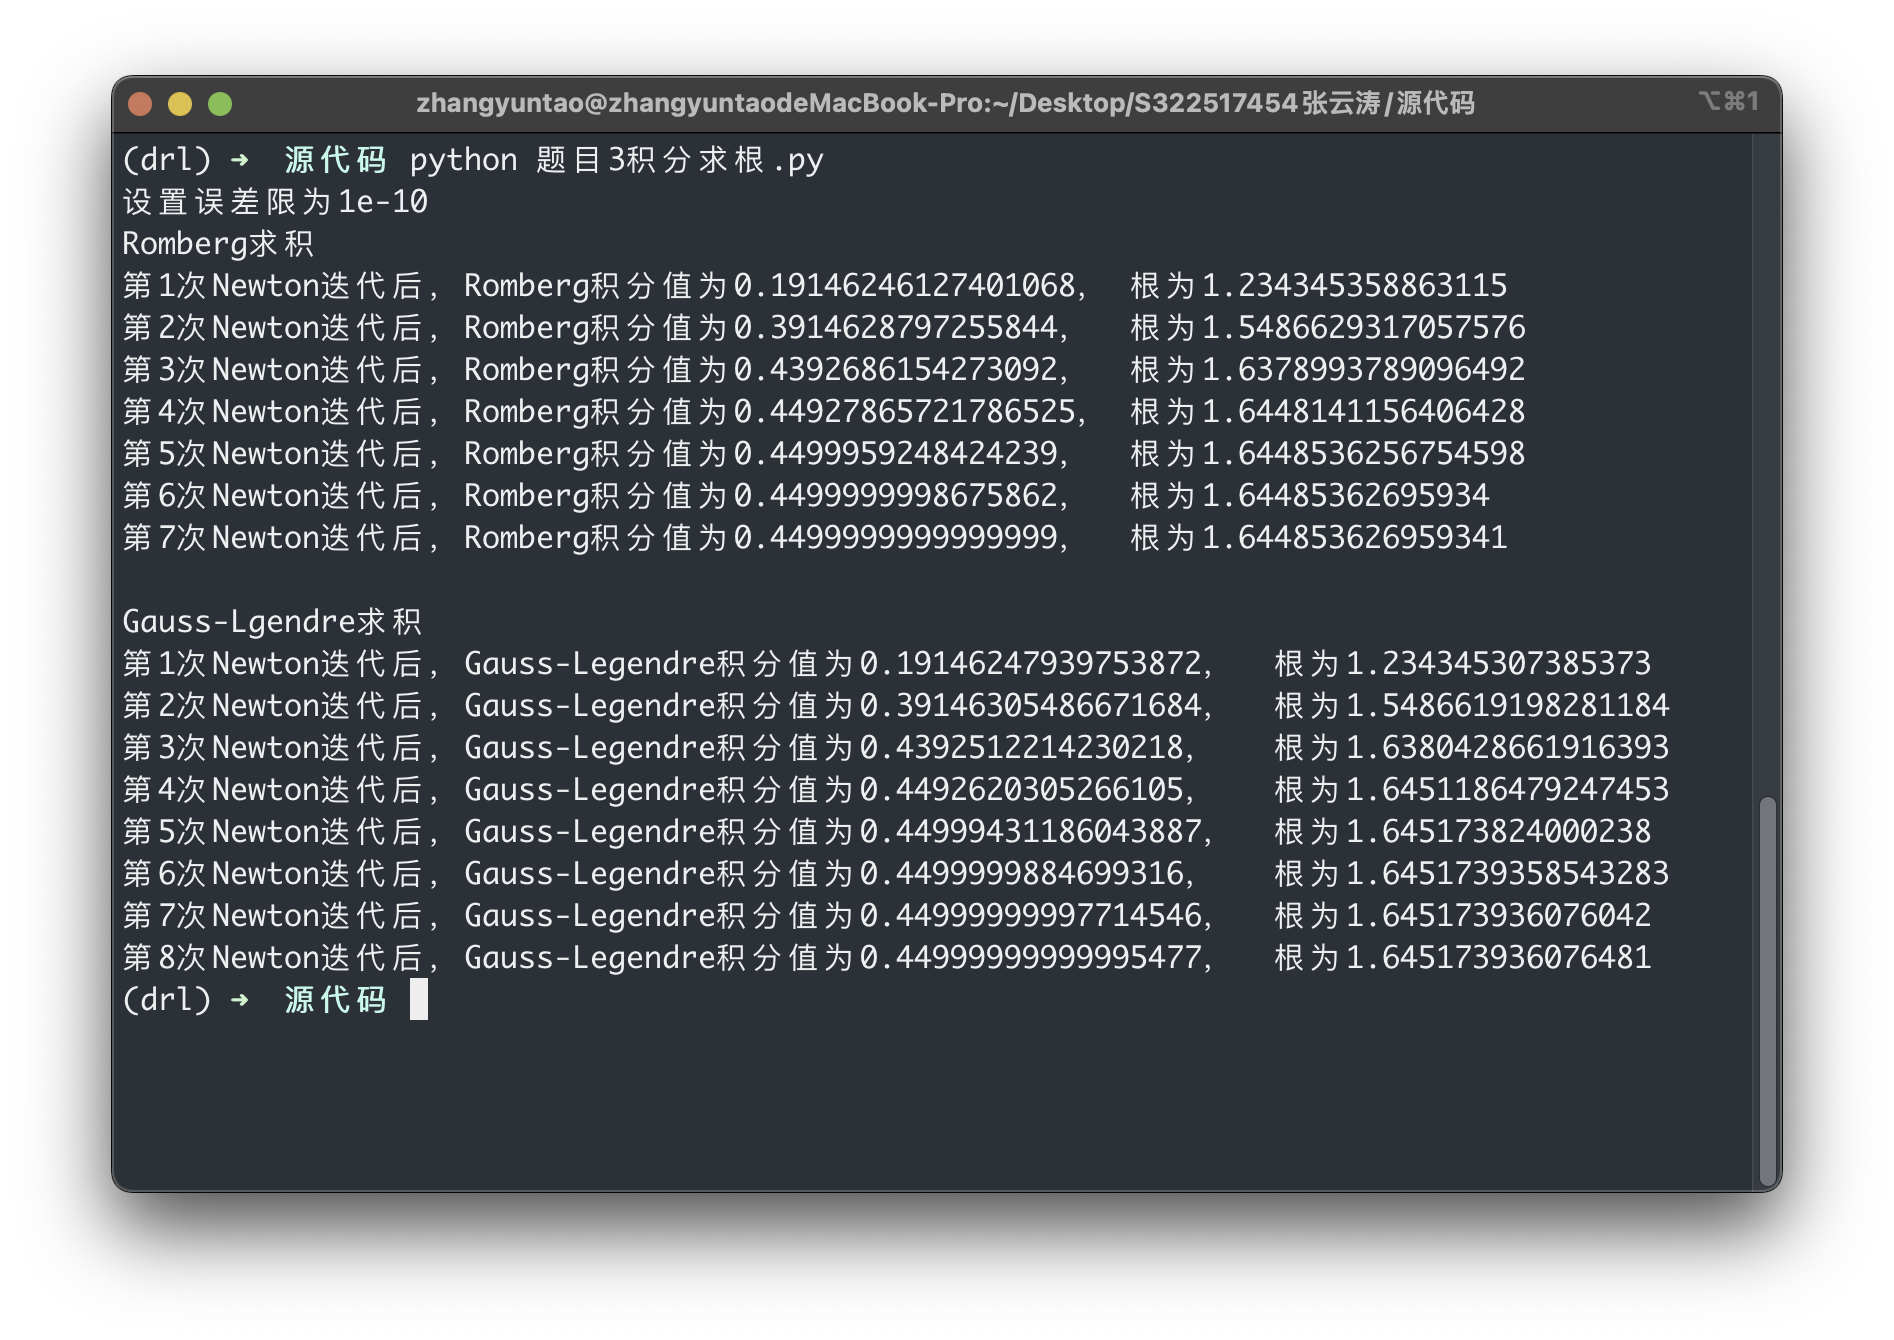
\includegraphics[width=\textwidth]{相关资源/图片/题目3运行结果.png} 
\end{figure}

设置误差限$e=1\times10^{-10}$,

Romberg求积 \\
第1次Newton迭代后,Romberg积分值为0.19146246127401068,	根为1.234345358863115; \\
第2次Newton迭代后,Romberg积分值为0.3914628797255844,	根为1.5486629317057576;\\
第3次Newton迭代后,Romberg积分值为0.4392686154273092,	根为1.6378993789096492;\\
第4次Newton迭代后,Romberg积分值为0.44927865721786525,	根为1.6448141156406428;\\
第5次Newton迭代后,Romberg积分值为0.4499959248424239,	根为1.6448536256754598;\\
第6次Newton迭代后,Romberg积分值为0.4499999998675862,	根为1.64485362695934;\\
第7次Newton迭代后,Romberg积分值为0.4499999999999999,	根为1.644853626959341;\\
最终解得根为1.644853626959341。\\

Gauss-Lgendre求积 \\
第1次Newton迭代后,Gauss-Legendre积分值为0.19146247939753872,	根为1.234345307385373;\\
第2次Newton迭代后,Gauss-Legendre积分值为0.39146305486671684,	根为1.5486619198281184;\\
第3次Newton迭代后,Gauss-Legendre积分值为0.4392512214230218,	根为1.6380428661916393;\\
第4次Newton迭代后,Gauss-Legendre积分值为0.4492620305266105,	根为1.6451186479247453;\\
第5次Newton迭代后,Gauss-Legendre积分值为0.44999431186043887,	根为1.645173824000238;\\
第6次Newton迭代后,Gauss-Legendre积分值为0.4499999884699316,	根为1.6451739358543283;\\
第7次Newton迭代后,Gauss-Legendre积分值为0.44999999997714546,	根为1.645173936076042;\\
第8次Newton迭代后,Gauss-Legendre积分值为0.44999999999995477,	根为1.645173936076481;\\
最终解得根为1.645173936076481。

\subsection{体会与收获}
通过此次编程实现,进一步掌握了
Romberg求积和
Gauss-Legendre求积
以及Newton迭代的方法。
尤其是手动实现Gauss-Lgendre求积的过程中,
因为忘记了系数$[\frac{5}{9},\frac{8}{9},\frac{5}{9}]$
这种细节问题,导致程序迟迟无法得到正常结果,
让我又一次得到了须认真的深刻教训。

%%%%%%%%%%%%%%%%%%%%%%%%%%%%%%%%%%%%%%%%%%%%%%%%%%%%%%%%%%%%%%%%%%%%%%
\newpage
\section{常微分方程初值问题}
% \setcounter{section}{4}
% \setcounter{subsection}{0}
\subsection{摘要}

2个分子的固态重镉酸钾(\ce{K_2Cr_2O_7})、
2个分子的水(\ce{H2O})和3个原子的固态硫磺(\ce{S})
结合生成3个分子的气态二氧化硫(\ce{SO2})、
4个分子的固态氢氧化钾(\ce{KOH})
和2个分子的固态氧化铬(\ce{Cr2O3})。 
此不可逆的化学反应可以由计量方程符号化地表示为
\begin{center}
    \ce{2K2Cr2O7 + 2H2O + 3S -> 4KOH + 2Cr2O3 + 3SO2} \\ 
\end{center}
如果$n_1$个分子的\ce{K2Cr2O7}、
$n_2$个分子的\ce{H2O}
和$n_3$个分子的\ce{S}最初是可以得到的,
下述的微分方程描述了在$t$时间后的数量$x(t)$。
\begin{equation}
    \frac{dx}{dt} = k(n_1-\frac{x}{2})^2(n_2-\frac{x}{2})^2(n_3-\frac{3x}{4})^3
\end{equation}
其中$k$是反应的速度常数。
如果,$k=6.22\times 10^{-19},n_1=n_2=2\times10^3, n_3=3\times10^3$,
则在0.2s后将形成多少单位的氢氧化钾?

\subsection{数学原理}
\begin{align}
    \text{四阶Runge-Kutta} & \nonumber \\
    y_{n+1} & = y_n + \frac{h}{6}(K_1+2K_2+2K_3+K_4) \\
    K_1 & = f(x_n, y_n) \\
    K_2 & = f(x_n+\frac{h}{2}, y_n+\frac{h}{2}K_1) \\
    K_3 & = f(x_n+\frac{h}{2}, y_n+\frac{h}{2}K_2) \\
    K_4 & = f(x_n+h, y_n+hK_3)
    \end{align}

\subsection{程序设计}
\lstinputlisting[language=Python,caption={from:源代码/题目4初值},captionpos=b, firstline=1, lastline=24]{源代码/题目4初值.py}

\subsection{结果分析}
通过调用scipy包使用四阶Runge-Kutta方法,
解得在0.2s后将形成2078.4446762377556单位的氢氧化钾。
\begin{figure}[H]
    \centering
    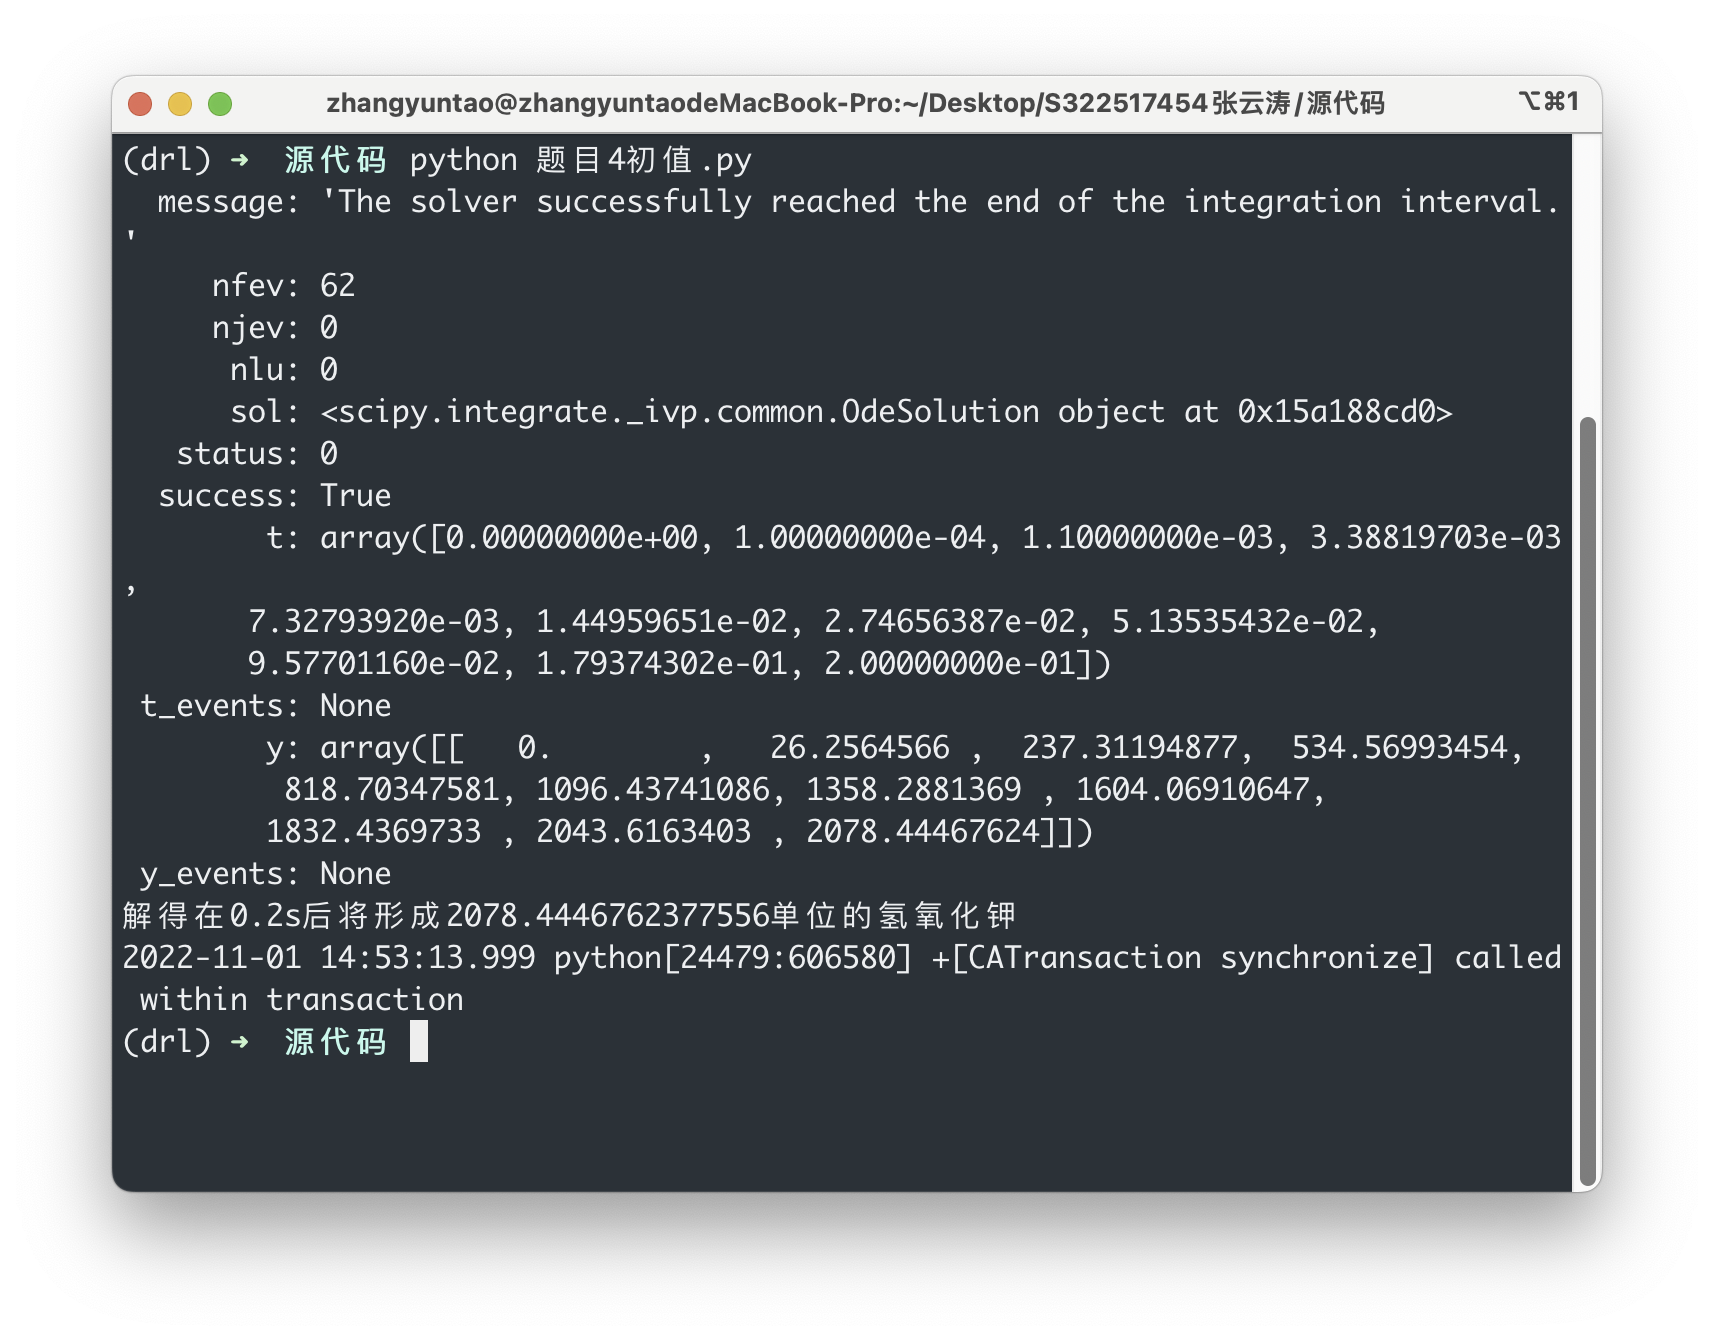
\includegraphics[width=\textwidth]{相关资源/图片/题目4运行结果1.png} 
\end{figure}
\begin{figure}[H]
    \centering
    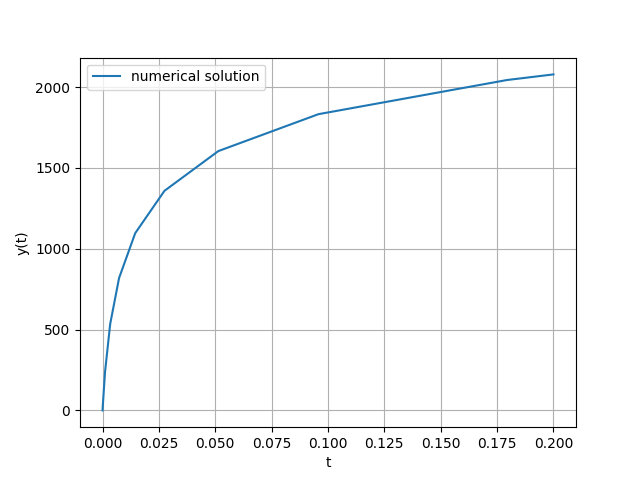
\includegraphics[width=\textwidth]{相关资源/图片/题目4运行结果2.png} 
\end{figure}

\subsection{体会与收获}
通过学习和实验,进一步掌握了使用四阶Runge-Kutta方法求解微分方程。
通过化学反应这一真实应用问题,切实感受到了数值计算方法的用处之大。
相信在今后的科研生活中,还会与数值计算为伴,
不断通过数值计算解决科研以及工作生活中遇到的各种难题。

%%%%%%%%%%%%%%%%%%%%%%%%%%%%%%%%%%%%%%%%%%%%%%%%%%%%%%%%%%%%%%%%%%%%
\newpage
\section{课程思政案例——插值算法在扫描软件中的应用。}
\subsection{摘要}

本项目为工业机器人智能喷涂项目,
为了实现对任意工件的智能喷涂,
需要先通过相机对工件进行扫描,
生成工件待喷涂面的深度图像,
进而分析图像规划喷涂方案。
\begin{figure}[H]
    \centering
    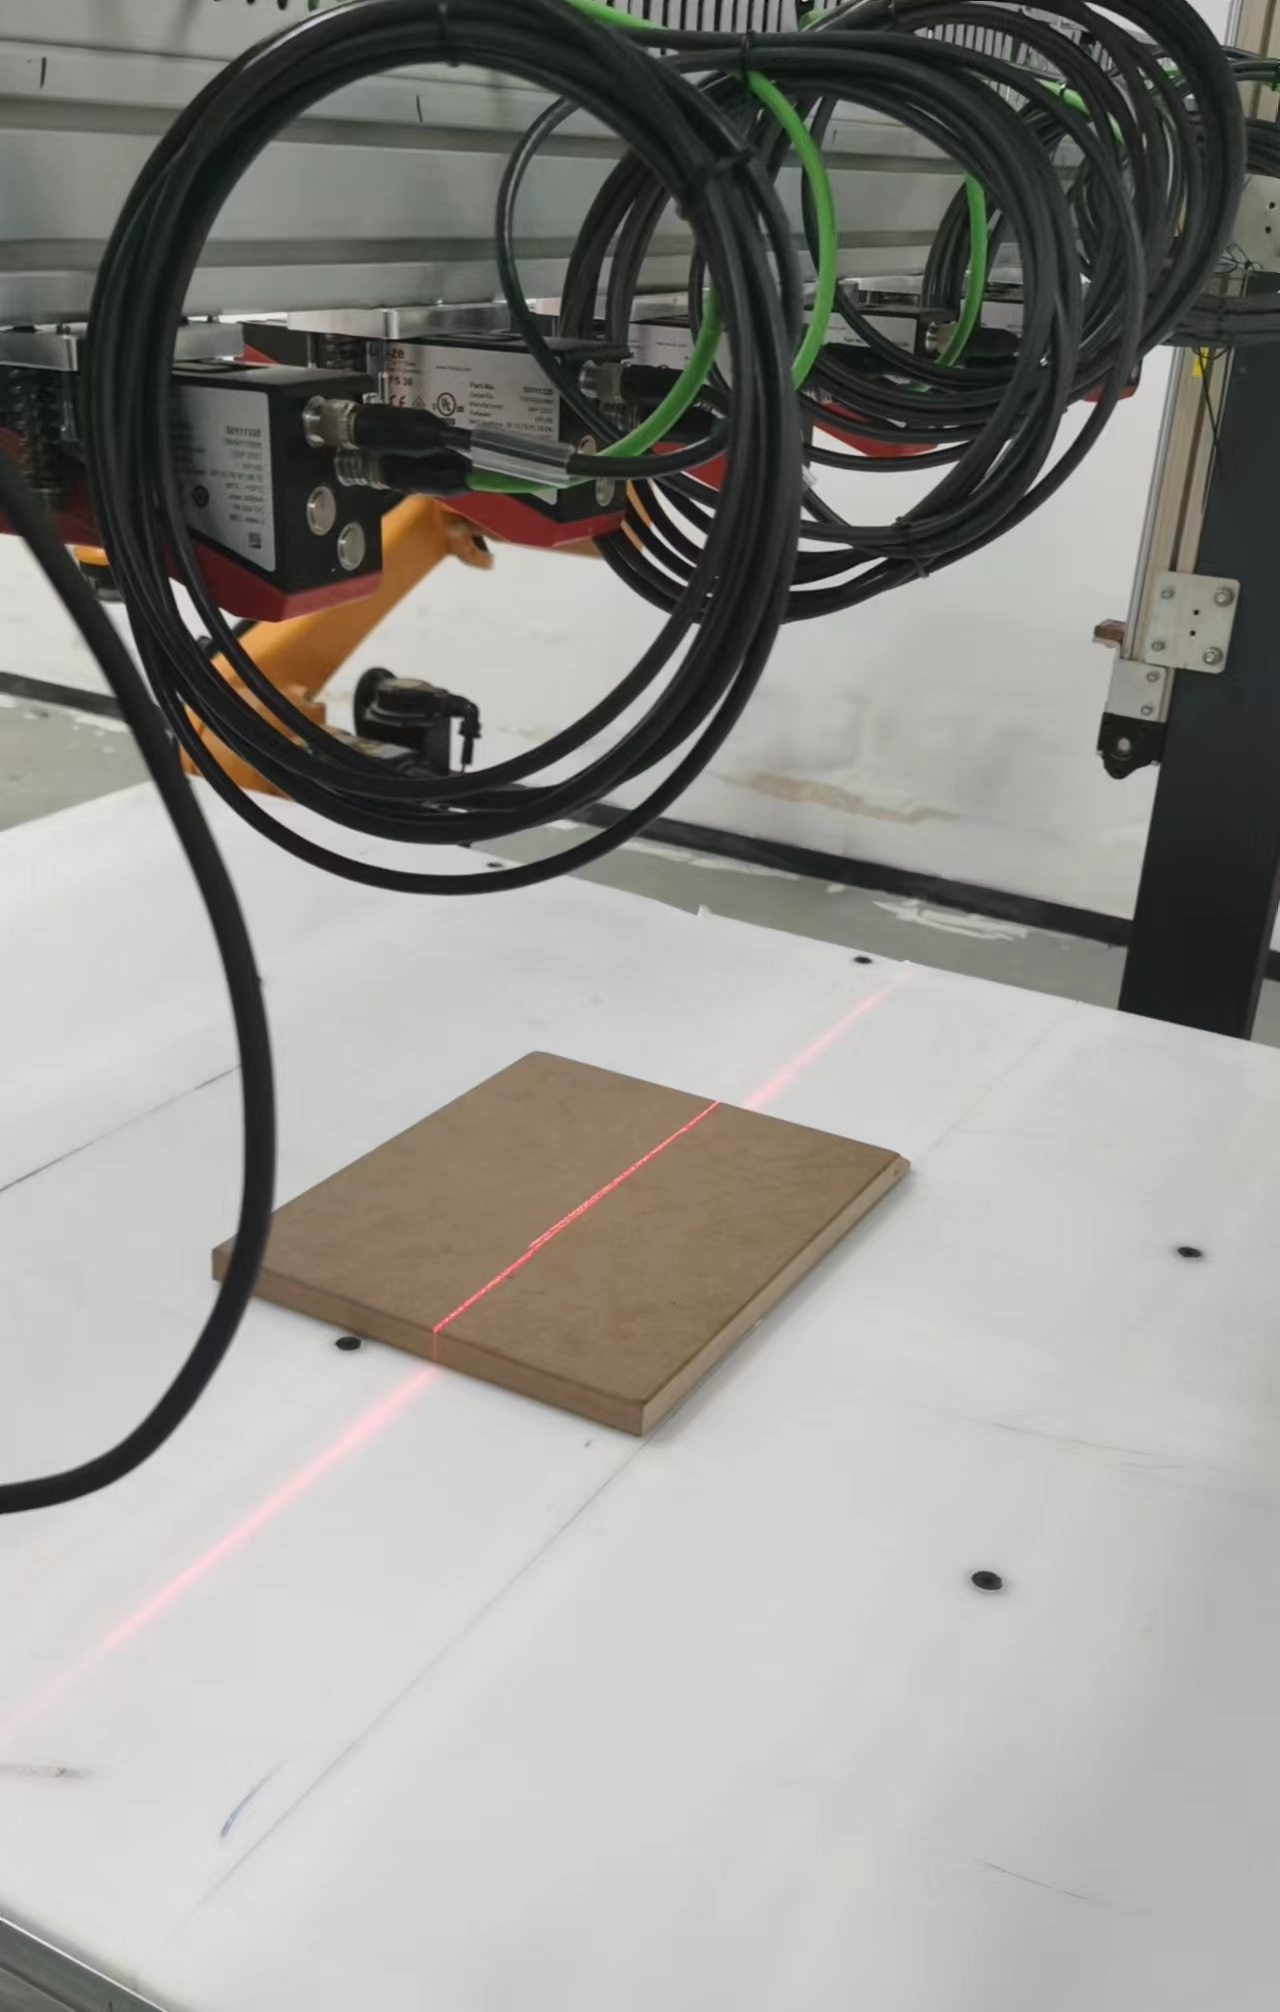
\includegraphics[width=\textwidth/2]{相关资源/图片/题目5扫描设备.jpg}  
\end{figure}
本项目中扫描方案如图所示,
因为每台相机能够测量的宽度有限,不能达到工件的宽度,
因此需要多台相机进行合作,
图中六台相机固定在一条直线上,
扫描通过六台激光相机获取的数据进行合成。 

每台相机通过发出激光,进行测距,每台相机返回投射到工件上的
距离信息,解析每台相机的数据,可以得到
一组含有256个距离点\verb|vector<x,z>|。
通过合成六台相机的数据,使之拼凑成一条直线,
以达到长度要求。

之后在下方传送带的移动过程中,相机不断获取深度信息,
最终得到一张深度图所需的足够的信息。

对数据进行插值,映射,最终生成一张深度图。

\subsection{数学模型或方程}
首先通过拼接六台相机一次获得的数据,得到一条线的数据,即一组\verb|VectorXZ|数据。
\begin{lstlisting}
VectorXZ CamGroup::Capture() {
    auto less_sort_point_x = [](std::pair<float, float> a, std::pair<float, float> b) -> bool {
        return a.first < b.first;
    };
    VectorXZ frame_;
    auto cam_cnt = ConfigManager::GetInstance()->GetCams().size();
    cout << "cams num: " << cam_cnt << endl;
    for(auto it:cam_v) {
        auto sub_frame_ = it->Capture();
        frame_.insert(frame_.end(), sub_frame_.begin(), sub_frame_.end());
        usleep(25000);
    }
    std::sort(frame_.begin(), frame_.end(), less_sort_point_x);
    // 插值
    auto res = tool::InterpolateXZ(1, frame_);
    return res;
}
\end{lstlisting}

之后,在下方传送带运动过程中,
加入y方向的信息,最终组成完整的图像信息\verb|VectorYXZ|。
\begin{lstlisting}
int LineManager::ScanThread() {
    float r = 1.0;
    //启动时清空存放的结果
    while(!scan_res_.empty())scan_res_.pop();
    //启动编码器
    if (scan_flag_ == true) {
        encoder_->StartRot();
    }
    while (scan_flag_ == true) {
        auto _frame_f = cam_group_->Capture();
        //判断是否存在相机连接断开
        if(_frame_f.size() < 10){
            controller_->error1_camerr();
            return 1;
        }else{
            //
            float _y_pos = encoder_->GetPosition();
            if (scan_res_.size() > 0){
                auto _frame0 = scan_res_.back();
                auto _frame1 = std::make_pair(_y_pos, _frame_f);
                auto _res = tool::InterpolateYXZ(1, _frame0, _frame1);
                for(size_t i=1; i<_res.size(); i++) {
                    scan_res_.push(_res[i]);
                }
            }else{    // 第一帧
                scan_res_.push(std::make_pair(_y_pos, _frame_f));
            }
            while (scan_res_.size() > q_scan_size_) {
                scan_res_.pop();
                cout << "POP" << endl;
            }
            int scan_duration_ = 5;
            if (scan_flag_){
                std::this_thread::sleep_for(std::chrono::milliseconds(scan_duration_));
            }else{
                encoder_->StopRot();
            }
            cout << endl;
        } 
    }
    return 0;
}
\end{lstlisting}

由于六台相机之间扫描的数据
有重合的部分,
导致x方向上的数据并不是均匀分布的。
因此需要通过\verb|InterpolateXZ()|进行插值。

在传送带匀速运动过程中,由于相机的通信时长限制,
y方向的数据并不能达到精度要求,
因此也要通过\verb|InterpolateYXZ()|对y方向进行插值。

\begin{lstlisting}[language=C++]
inline std::vector<std::pair<float, float> > InterpolateXZ(float inter_val, std::vector<std::pair<float, float> > src_data) {
    std::vector<std::pair<float, float> > inter_cap = {src_data[0]}; // 先插入第一点
    std::vector<double> _frame_x, _frame_z;
    _frame_x.clear();
    _frame_z.clear();
    auto last_x = src_data[0].first;
    for(size_t i=1; i<src_data.size(); i++) {
        if (src_data[i].first > last_x) {
            _frame_x.push_back(src_data[i].first);
            _frame_z.push_back(src_data[i].second);
            last_x = _frame_x.back();
        }
    }
    // 三次样条插值
    tk::spline s;
    s.set_points(_frame_x, _frame_z);
    float p_0 = _frame_x[0];
    double p_end = _frame_x[_frame_x.size()-1];
    for(auto p=p_0+inter_val; p<p_end; p+=inter_val) {
        float p_z = s(p);
        auto _point = std::make_pair(p, p_z);
        inter_cap.push_back(_point);
    }
    return inter_cap;
}

typedef std::vector<std::pair<float, float> > VectorXZ;    
inline std::vector<std::pair<float, VectorXZ> > InterpolateYXZ(float interval, std::pair<float, VectorXZ> frame0, std::pair<float, VectorXZ> frame1) {
    std::vector<std::pair<float, VectorXZ> > inter_res;
    float _inter_y = frame0.first;
    while (_inter_y <= frame1.first) {
        float a = _inter_y;     // 返回第一帧
        VectorXZ _frame;
        for(size_t i=0; i<frame1.second.size(); i++) {
            auto _point = (frame1.second)[i];
            auto _prev_point = (frame0.second)[i];
            // float b = _point.second;
            float b = (_point.second-_prev_point.second)/(frame1.first-frame0.first)*(a-frame0.first) + _prev_point.second;
            _frame.push_back(std::make_pair(_point.first, b));  // x-z
        }
        _inter_y += interval;
        inter_res.emplace_back(a, _frame);     // y-(x-z)
    }
    return inter_res;
}
\end{lstlisting}

最终通过x和y方向的插值,得到一张点均匀分布的深度图像。

\subsection{数值求解}

最终生成扫描结果如下图所示的图片,用于下一步的生产处理。
\begin{figure}[H]
    \centering
    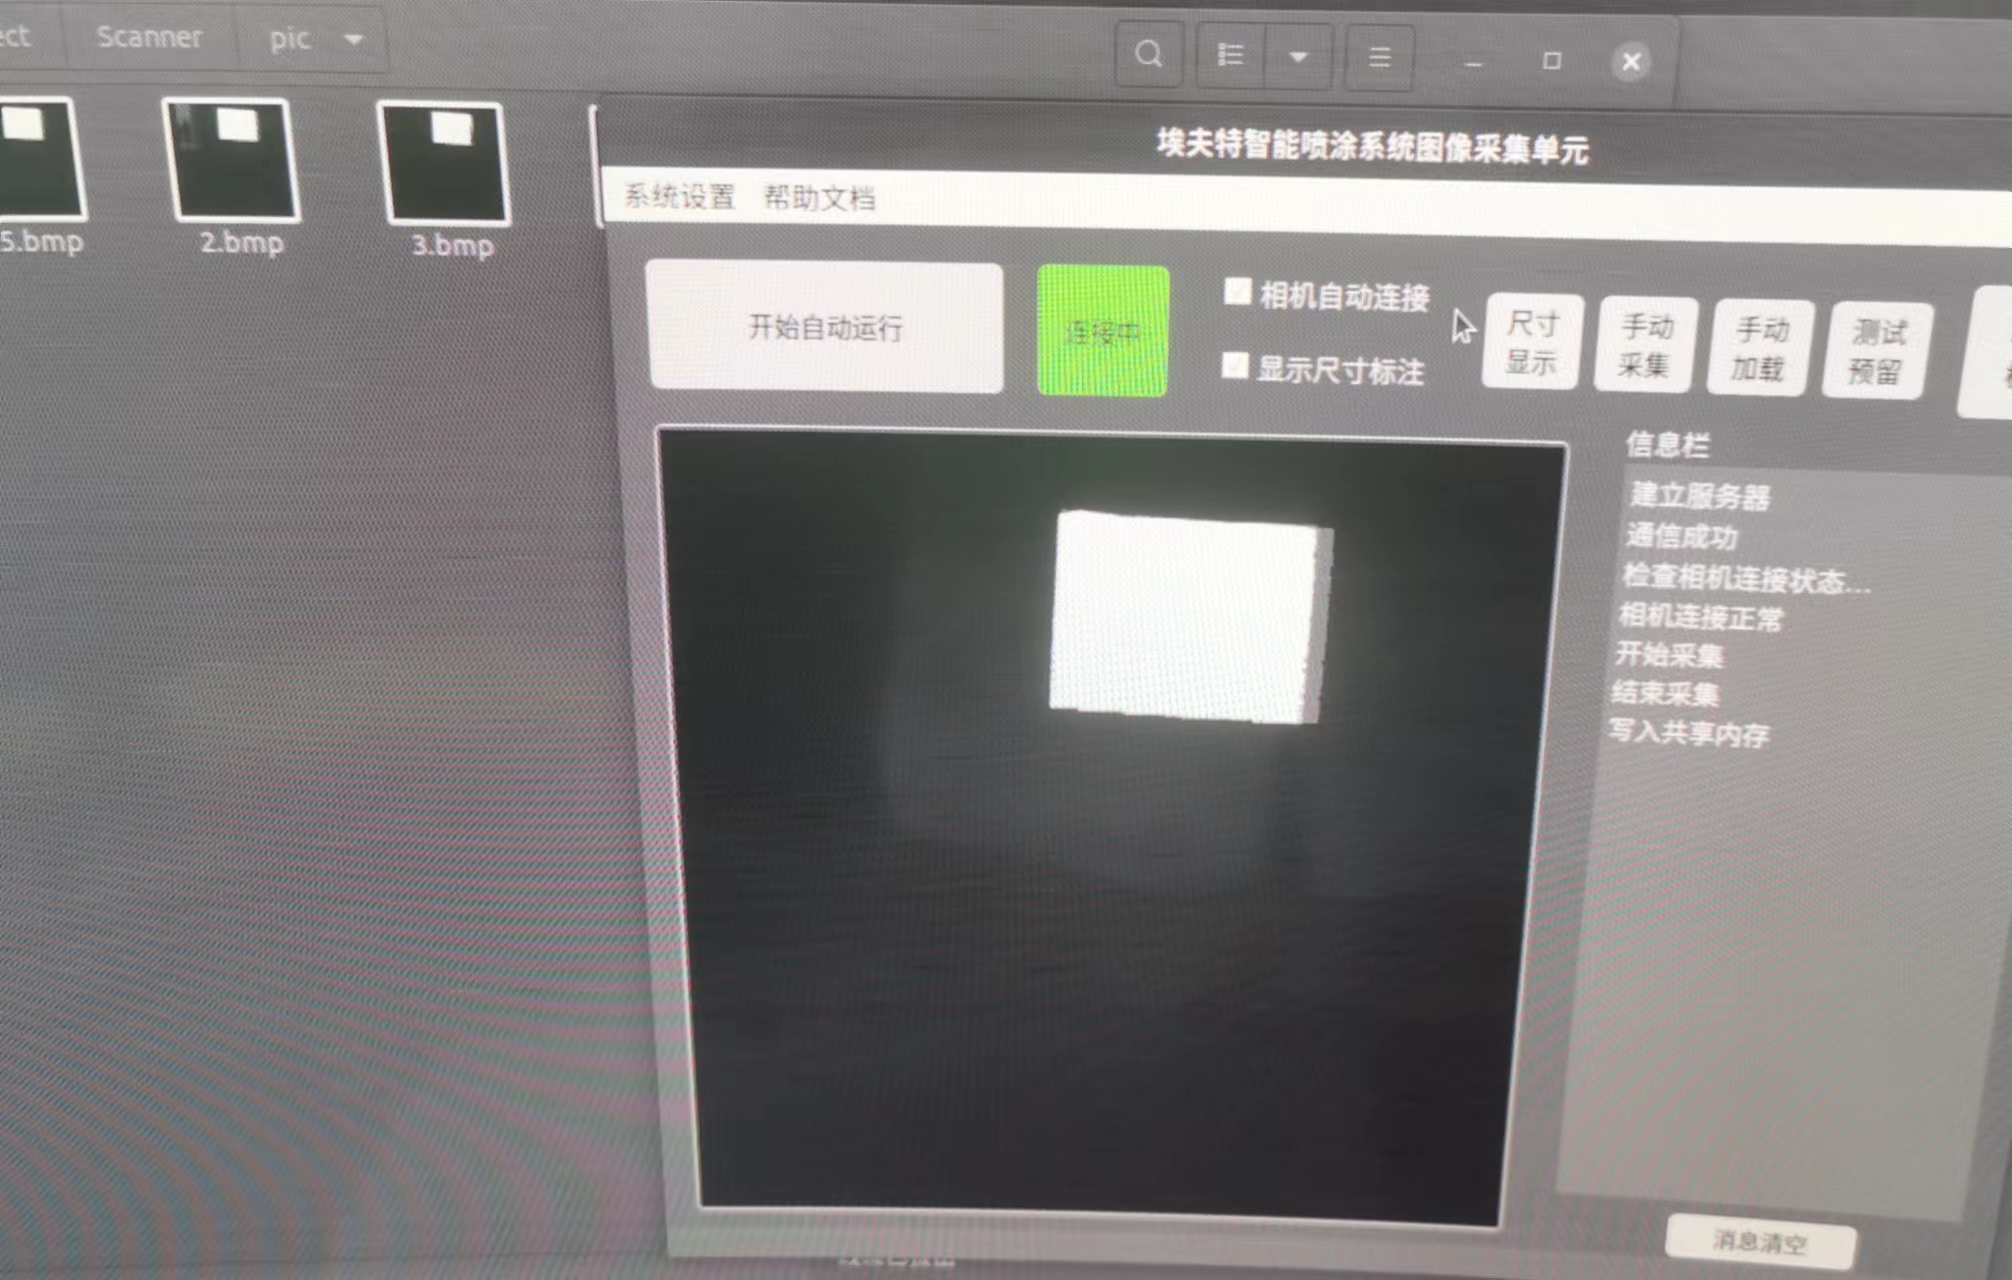
\includegraphics[width=.8\textwidth]{相关资源/图片/题目5扫描结果.jpg}  
\end{figure}
以数据文件夹中存储的一次扫描结果为例,
扫描结果部分数据如下表所示,完整数据可参考
文件“数据/题目5扫描结果数据.csv”。
\begin{table}[H]
    \centering
    \begin{tabular}{|l|l|l|l|}
    \hline
        0 & 0 & -4.2 & 499.6 \\ \hline
        0 & 1 & -4.2 & 499.6 \\ \hline
        0 & 2 & -3.2 & 499.055 \\ \hline
        0 & 3 & -2.2 & 499 \\ \hline
        0 & 4 & -1.2 & 499.073 \\ \hline
        0 & 5 & -0.199997 & 499.158 \\ \hline
        0 & 6 & 0.800003 & 499.155 \\ \hline
        0 & 7 & 1.8 & 499.064 \\ \hline
        0 & 8 & 2.8 & 499.136 \\ \hline
        0 & 9 & 3.8 & 499.464 \\ \hline
        0 & 10 & 4.8 & 499.292 \\ \hline
        0 & 11 & 5.8 & 499.208 \\ \hline
    \end{tabular}
\end{table}

\subsection{结果分析}
通过分析上表中数据,并可视化
\begin{figure}[H]
    \centering
    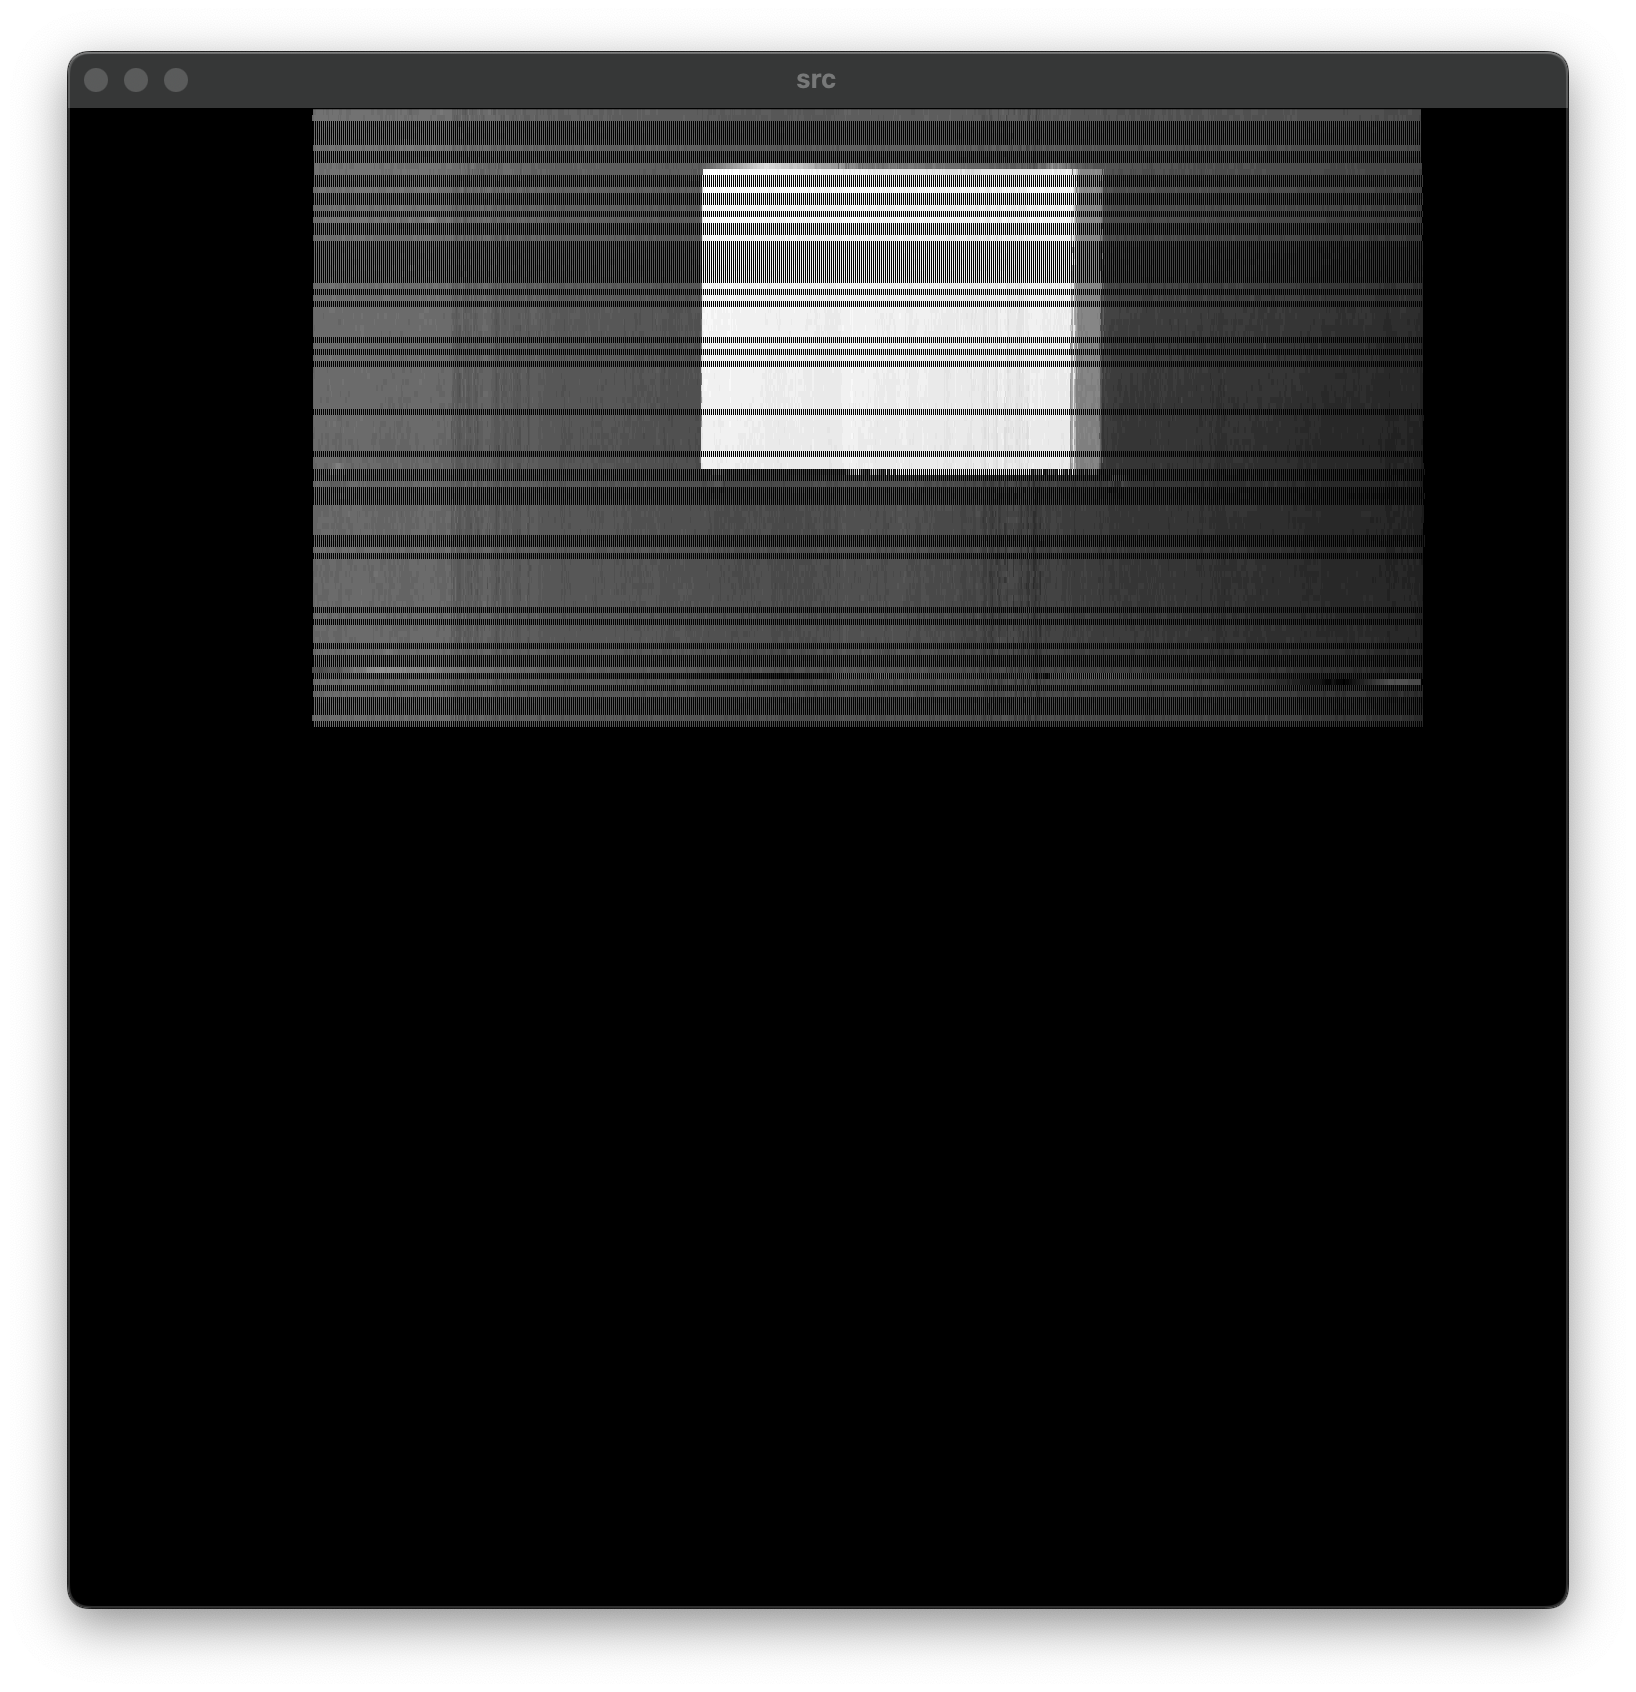
\includegraphics[width=.5\textwidth]{相关资源/图片/题目5扫描结果分析.png} 
\end{figure}
可以看出插值后的数据均匀分布。

\subsection{具体应用方向}
本扫描软件已经成功应用于喷涂项目中,也可以作为一个独立软件,
以适应其他场景的需求。

\subsection{相关心得}
数值分析的算法实际应用非常广泛,在工作中,经常会用到
各种相关算法。
通过在这次的喷涂项目中使用到插值算法,更能切实感受到
数值分析的重要性。

\vspace*{2cm}
\copyright~张云涛 https://github.com/jonty-zh/numerical-analysis-homework

\end{document}